This research analyzes the current scenario and future implications of autonomous driving systems, addressing the creation process of a user interface able to communicate intentions and movements of autonomous vehicle.
The ultimate goal is to increase the confidence felt by the user to this system, encourage inclusion, acceptance and all the benefits it could bring to user mobility, and emotions.
We envision a scenario in which car is not only a tool to get from point A to point B, but a complex device that receives and provides information, is connected to the network, knows traffic situation, programs maintenance, can recognize emotional states, hypothetical distractions and driver physical problems (sleep or tiredness), is able to teach the correct way to drive through feedback and, vice-versa, learning input from the driver.
\begin{wrapfigure}{r}{0.45\textwidth}
  \begin{center}
    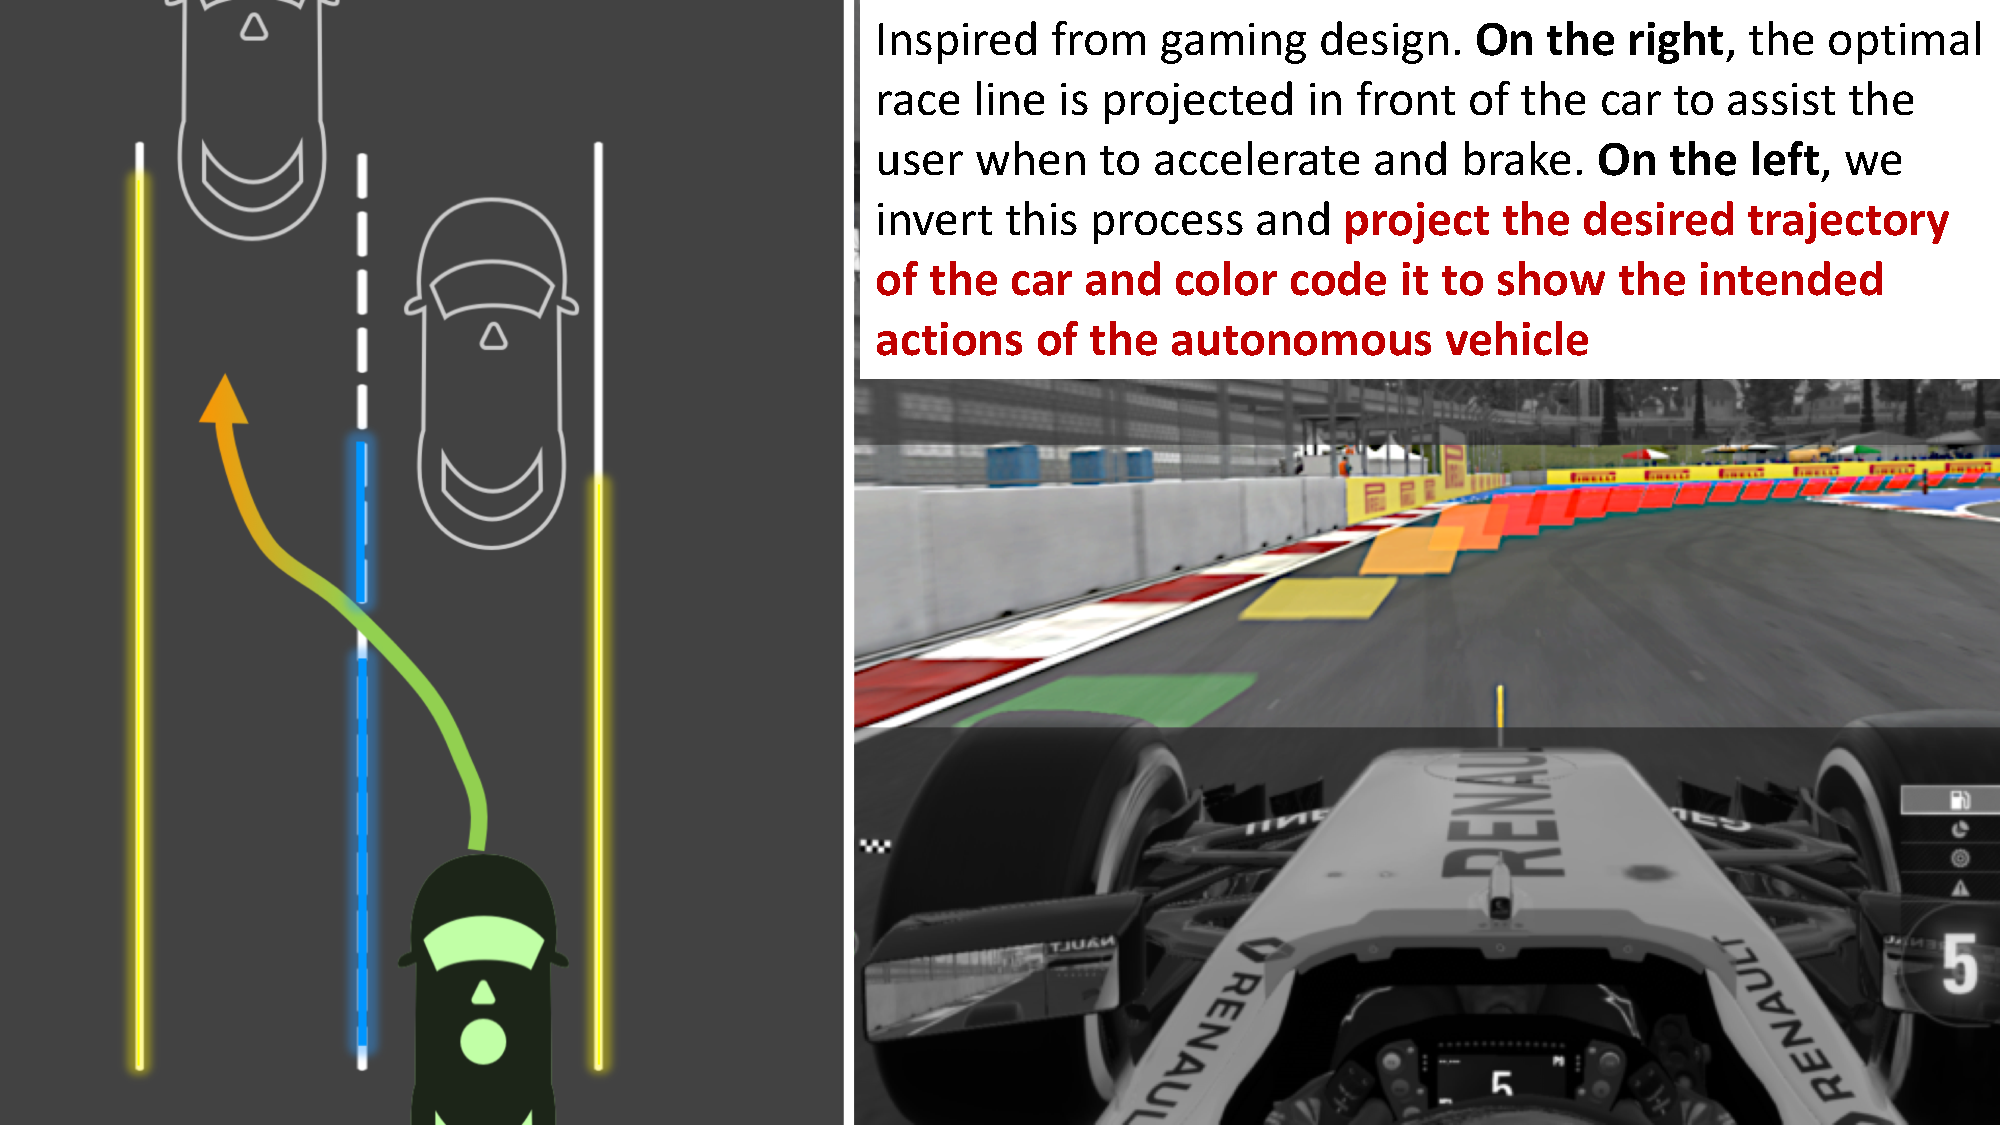
\includegraphics[width=0.43\textwidth]{figures/trajectory_ui.pdf}
  \end{center}
  \caption{Inspired from gaming, projecting the intended trajectory of the car in a color coded manner can realy critical feedback to the user about what actions the car intends to take in any given situation.}
  \label{fig:trajectory}
\end{wrapfigure}
Graphical user interface is an essential tool to create a bridge between the passenger and the autonomous vehicle. 
Present day dashboards/instrument clusters/user interface for semi autonomous vehicles present a high level overview or a wireframe view of what the car sees as its driving. Its typical to highlight lane markings and road signs, and even highlight potential hazards.
However, what is lacking is a design to transparently communicate the intended actions of the vehicle. 
Such transparency is important, because the algorithms by which autonomous cars make decisions are largely invisible to the driver.
If something unexpected occurs, the driver can only speculate what happened. In Section~\ref{subsec:explainability}, we presented an approach to explain the car's actions when driver distress, or a hard braking/steering event occurs. 

In our autonomous vehicle simulator, we will test graphical interfaces design which convey the intention of the autonomous car to the passenger. We are not proposing designing production ready user interfaces for autonomous cars, but a functional study for testing, determining visual variables complexity, information hierarchy and topology, and cognitive load for certain functional UI elements. 
Think of it as a `visual storyboard' of what is happening outside the car. The UI elements will show immediate future movements and choices. ``\textit{Why is the car turning right?}'', ``\textit{Which way is it taking?}'', ``\textit{Can the car detect the cyclist in front of me?}''.
The interface is based on two fundamental principles: simplicity (of use) and anthropomorphism (of language). 
It's not designed for an audience of engineers or designers, it is designed to be as simple as possible, usable and understandable by anyone.

To present a example, we take inspiration from design for motorsport gaming. As shown in Figure~\ref{fig:trajectory}(right), many games project a path in front of the race car to guide the user which is the fastest race line on the track. The color of the race track tells the gamer where to accelerate (green) or slow down (amber). Our idea is to invert this concept for an autonomous car where the UI (Figure~\ref{fig:trajectory}(left)) shows the intended trajectory of the autonomous vehicle and the color of the trajectory coveys if the car will speed up of slow down (brake). We hypothesize that such feedback can help passengers gauge their ``predictability'' metric and hence teir confidence, and trust in the vehicles. 
